\question{Câu 6}

Cho một tín hiệu cần xử lý dưới dạng điện áp, có tầm thay đổi từ $10\,\textsf{mV} - 30 \,\textsf{mV}$.  

\answer{a}{Thiết kế mạch khuếch đại tín hiệu lên 100 lần.}

Vẽ sơ đồ đặc tuyến ngõ vào và ngõ ra của mạch theo yêu cầu như sau:

\begin{figure}[H]
	\centering
	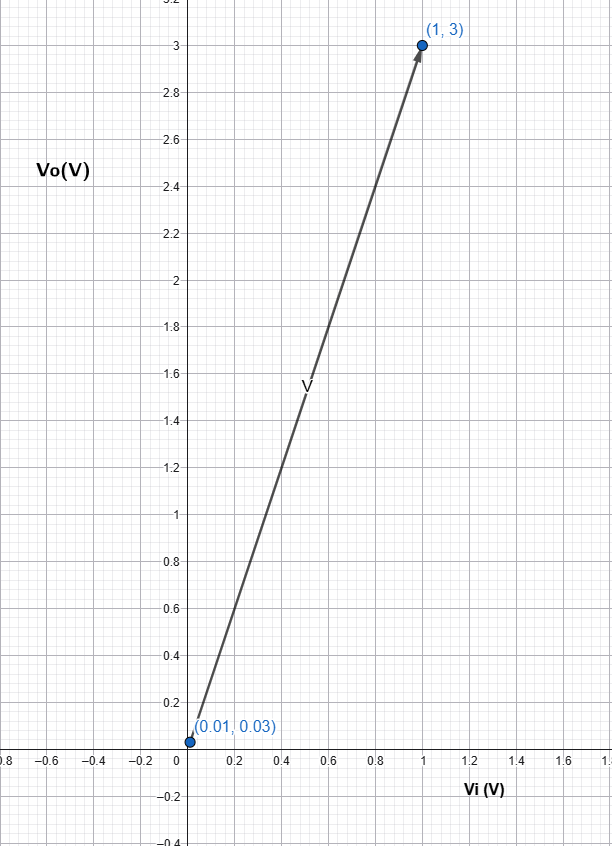
\includegraphics[width=.3\linewidth]{./my-chapters/my-images/Question6/debai_sododienap.png}
\end{figure}

Nhóm em quyết định sử dụng mạch Khuếch đại không đảo (The Non-inverting Amplifier) bởi vì:

\begin{itemize}[label=-]
	\item Có ngõ ra không bị đảo so với ngõ vào.
	\item có điện trở ngõ vào ($R_{in}$) rất lớn.
	\item Tuy nhiên sẽ hơi khó chọn giá trị $R_{1}$ và $R_{2}$.
\end{itemize}

\begin{figure}[H]
	\centering
	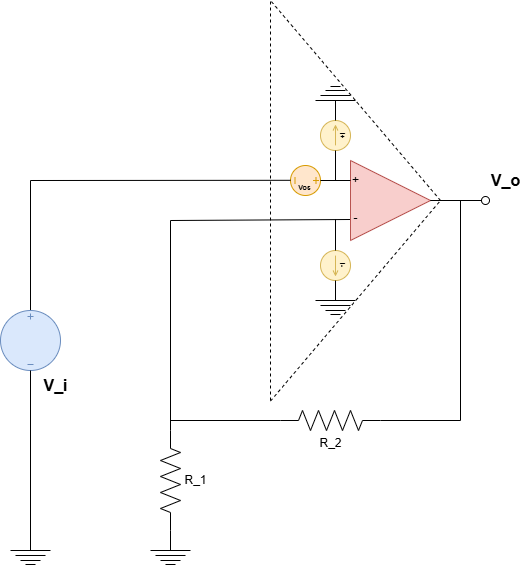
\includegraphics[width=.7\linewidth]{./my-chapters/my-diagrams/Question5/a_non-ideal-module.png}
	\caption{Sơ đồ mạch tương đương.}
\end{figure}

\begin{itemize}[label=-]
	\item Xét $V_{in}$, $V_{os} = 0$, $I_{+} = 0$, $I_{-} = 0$:
	\[ V_{out} = \left( 1+ \dfrac{R_{2}}{R_{1}}\right) V_{in} \]
	\item Xét $V_{os}$, $V_{in} = 0$, $I_{+} = 0$, $I_{-} = 0$:
	\[ V_{out} = \left( 1+ \dfrac{R_{2}}{R_{1}}\right) V_{os} \]
	\item Xét $I_{+}$ và $I_{-}$, $V_{in} = 0$, $V_{os} = 0$:
	\[ V_{out} = I_{-}R_{2} \]
\end{itemize}
$\Rightarrow V_{out} = \left( 1+ \dfrac{R_{2}}{R_{1}}\right) V_{in} + \left( 1+ \dfrac{R_{2}}{R_{1}}\right) V_{os} + I_{-}R_{2}$

\answer{b}{Lựa chọn OPAMP và các linh kiện cần thiết để thực hiện mạch hoạt động.}

Ta xét,

\begin{itemize}[label=-]
	\item \textbf{Chọn hệ số khuếch đại của mạch (Gain):} Để có $V_{out} = 100\times V_{in} \Rightarrow A_{v} = \left( 1+ \dfrac{R_{2}}{R_{1}}\right) = 100$
	$\Rightarrow
	\left\{
	\begin{matrix}
		R_{1} = 3.3\,\textsf{k}\Omega \\[4pt]
		R_{2} = 330\,\textsf{k}\Omega
	\end{matrix}
	\right.
	$
	
	$\rightarrow A_{v} = \left( 1 + \dfrac{R_{2}}{R_{1}} \right) = 101 \,\textsf{V/V}$
	\item \textbf{Output swing và supply rails:} Với ngõ ra rơi vào tầm $1-3\,\textsf{V}$ thì chọn nguồn từ $0\rightarrow 5\,\textsf{V}$ hoặc $\pm5\,\textsf{V}$ trở đi là được.
	
	\item \textbf{Input offset và Noise:} $\Delta V = \left( 1+ \dfrac{R_{2}}{R_{1}}\right) V_{os} + I_{-}R_{2}$
		\begin{itemize}[label=+]
			\item $V_{os}$ phải đủ nhỏ rơi vào tầm $\mu\,\textsf{V}$ để $V_{out} = \left( 1+ \dfrac{R_{2}}{R_{1}}\right). V_{os} \approx \textsf{mV}$
			\item $I_{-} = \left\{ \begin{matrix}
					\dfrac{1}{2}I_{os} - I_{ib} \\[4pt]
					\dfrac{1}{2}I_{os} + I_{ib}
				\end{matrix} \right.$ thì phải chọn $|I_{os}| < |I_{ib}|$ rơi vào \textsf{nA}.
		\end{itemize}
%	\item \textbf{Slew rate (SR):} thể hiện đáp ứng thay đổi của ngõ ra có thể thay đổi 
\end{itemize}

Từ đó, nhóm em chọn OPAMP: \href{https://www.ti.com/lit/ds/symlink/opa277.pdf?ts=1761750470596&ref_url=https%253A%252F%252Fwww.mouser.com%252F}{\textbf{OPA277U}}.

\begin{figure}[H]
	\centering
	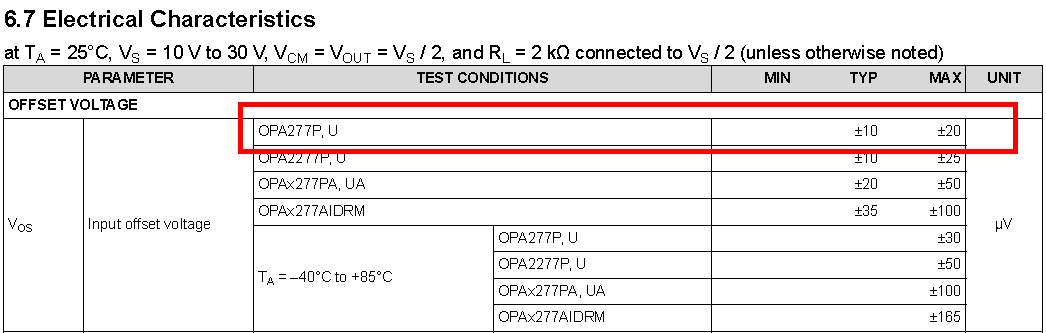
\includegraphics[width=.9\linewidth]{./my-chapters/my-images/Question6/V_os_opa277u.pdf}
	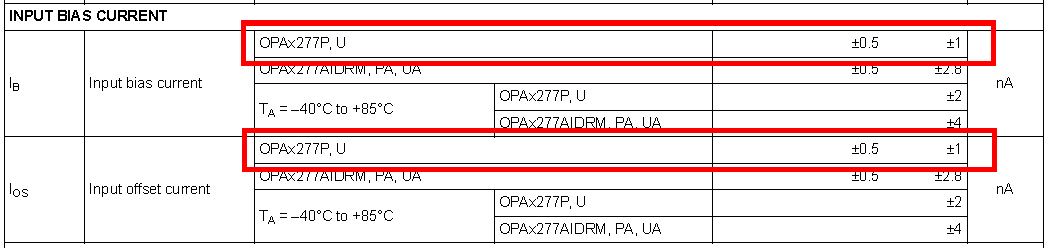
\includegraphics[width=.9\linewidth]{./my-chapters/my-images/Question6/I_os_I_ib_opa277u.pdf}
	\caption{Electrical Characteristics for OPA227U.}
\end{figure}